\documentclass[]{thesis}  % draft mode (default)
%\documentclass[review]{thesis}  % review mode (show contents & reference only)
%\documentclass[watermark,final]{thesis}  % final mode (version for library)

%-------------------------------------------------------------------------------
% Package Loading
%-------------------------------------------------------------------------------

\usepackage{multirow}     % for multi-row table
\usepackage{booktabs}     % table style used in books
\usepackage[shortlabels]{enumitem}
%-------------------------------------------------------------------------------
% Configuration
%-------------------------------------------------------------------------------

% 填寫題目, 作者, 指導教授, 學校, 系所, 日期等資訊
% Title
\title{ Blockchain-based Identification and Access Control for Open Banking Ecosystem}
\titlezh{基於區塊鏈的身份識別與存取控制用於開放銀行}

% Author
\author{Jen-Hao Cheng}
\authorzh{鄭人豪}

% Advisor
\advisor{Shyan-Ming Yuan}
\advisorzh{袁賢銘}

% First co-advisor (Leave {} empty if you don't have a co-advisor)
\coadvisorA{}
\coadvisorAzh{}

% Second co-advisor (Leave {} empty if you don't have a second co-advisor)
\coadvisorB{}
\coadvisorBzh{}

% Field
\field{Computer Science}

% Institute
\institute{Institute of Network Engineering}
\institutezh{網路工程研究所}

% College
\college{College of Computer Science}

% University
\university{National Chiao Tung University}
\universityzh{國立交通大學}

% Location
\location{Hsinchu, Taiwan}

% Date of final submission
\degreemonth{Sep}
\degreeyear{2021}
\degreeyearzh{中 華 民 國 110 年 7 月}

% Watermark
\watermark{figures/nctu_logo.jpg}

% 修改 thesis.cls 的預設字型
%-------------------------------------------------------------------------------
% Chinese Font Settings
%
%   These macros are used to change the default Chinese fonts (see below) used
% by thesis.cls. Please leave {} empty if you want to use the default settings
% and make sure that you have added '-shell-escape' option when using xetex to
% compile tex files, i.e. xetex compiling commands should run something like:
%
%     xelatex -synctex=1 -shell-escape -interaction=nonstopmode %.tex
%
% (default Chinese font settings)
%   Windows              Linux                        Mac OS X
% * 標楷體 (DFKai-SB)    AR PL 中楷 (AR PL UKai TW)   楷體-繁 (Kaiti TC Regular)
% @ 新細明體 (PMingLiU)  AR PL 明體 (AR PL UMing TW)  儷宋 Pro (LiSong Pro)
%
% * fontname --> 預設中文本文字型 (serif)
% @ fontname --> 預設中文明體字型 (sans-serif, 使用於封面頁)
%-------------------------------------------------------------------------------

% main (serif) Chinese font, leave {} empty to enable default font setting
\mainfontzh{}

% sans-serif Chinese font, leave {} empty to enable default font setting
\sansfontzh{}

%-------------------------------------------------------------------------------
% English Font Settings
%
%   These macros are used to change the default English fonts (see below) used
% by thesis.cls. Please leave {} empty if you want to use the default settings.
%
% (default English font settings)
% main font       --> Times New Roman (for all platforms)
% sans-serif font --> Arial           (for all platforms)
%-------------------------------------------------------------------------------

% main font for English, leave {} empty if you want to use default font setting
\mainfont{}

% sans-serif font for English, leave {} empty if you want to use default setting
\sansfont{}



\begin{document}

% Show repeated author names in bibliography when using IEEEtran.bst
% Comment out this line if you don't set IEEEtran in \bibliographystyle{}
\bstctlcite{IEEEexample:BSTcontrol}

% Generate cover, title, authorization, approval and copyright pages
\maketitle

%-------------------------------------------------------------------------------
% Abstract
%-------------------------------------------------------------------------------

% 中文摘要
\begin{abstractzh}

    隨著社群平臺愈來愈普及,多數網站提供第三方登入(social login),讓初次使用的用戶可以用第三方平臺現有的帳號完成註冊及登入,
    幫助用戶免於記下不同網站的帳號及密碼,亦不用填寫繁雜的註冊表單。對於用戶而言,可以達到更好的用戶使用體驗;對於應用程式開發人員而言,不必自行管理個資、建立會員系統,由第三方平臺負責管理,而當需要在提供多種不同的服務時,可以使這些服務支援同一種第三方平臺驗證方式,即可達到單一登入(SSO)功能。但第三方登入系統仍屬於中心化系統,用戶的數位身分及資料皆屬於第三方平臺,因此用戶在使用服務的同時,也提供個人資料給服務提供者。\par
    然而,以太坊區塊鏈擁有防偽造、防竄改及去中心化的特性,可以安全、有效存放紀錄於鏈上,達到透明性且安全性。透過以太坊虛擬機及以太坊智能合約可以建構去中心化的應用程式,提供更完整、多樣的功能。\par
    本篇論文提出使用以太坊區塊鏈技術應用於開放銀行(Open Banking),使銀行機構與第三方服務業者(TSP)以安全、透明方式合作,透過區塊鏈技術管理並整合用戶身分,方便用戶管理及存取資料,且提供第三方登入的優點,並使得去中心化平臺成為信任的第三方,負責管理對應用戶身分並且提供存取控制之功能,同時兼具區鏈特性,提升安全性。除了驗證用戶身分功能外,亦提供用戶授權功能,用戶可以自行決定授權範圍及對象,授權對象包含第三方服務(TSP)業者。

\end{abstractzh}

\begin{flushleft}
    \textbf{關鍵字}: 區塊鏈、智能合約、第三方服務提供者、開放銀行
\end{flushleft}

% 英文摘要
\begin{abstract}%

    Open Banking has become a trend in the financial industries for providing innovative and diverse services. The concept of open banking aims to give providers access to customer's financial data securely, thereby helping customers and third-party service providers (TSP) get a better deal and experience. Since an open banking ecosystem serves as a platform for various participants, identity verification and access control management are high priorities. When the bank reveals application programming interfaces to TSP's, the security issues are identity theft, data tampering. The objective of our research was to formulate the protocol flow that blockchain-based identification and account integration. That makes our customers securely access their data and authorize TSP to access their data. In addition to authorization,  they don't need a centralized server to manage their contract for deciding whether disclose data. We used the Ethereum blockchain to implement the system prototype to realize that data sharing and access control management. Our experiment results show the scalability and usability of our system prototype.\par

\end{abstract}

\begin{flushleft}
    \textbf{Keywords}: Blockchain, Smart contract, Third-party providers, Open banking
\end{flushleft}

%-------------------------------------------------------------------------------
% Acknowledgement
%-------------------------------------------------------------------------------

% 誌謝
\begin{acknowledgement}%

    非常高興能夠完成碩士班學業,這段經歷是我求學生涯中,最讓我刻骨銘心,畢生難忘的。在這兩年的學習與研究裡,碩士論文能夠如期完成,要感謝許多人的幫助,在此獻上敬意。

    首先誠摯感謝我的指導教授 \underline{袁賢銘}老師,老師的悉心教導使我能夠一窺研究領域的深奧,也在研究過程中,不厭其煩地給予指導與協助,提供完整的研究資源;老師開明又親和的指導風格也我深感佩服與尊敬,也使我在這兩年獲益匪淺,更是我一生學習的典範。另外,感謝口試委員\underline{黃彥男}教授、\underline{梁德容}教授、\underline{張玉山}教授於口試時給予寶貴的建議及指教,使我的研究更趨於完善。
    
    再來感謝實驗室夥伴\underline{廷翰}、\underline{城溥}、\underline{佳儀}、\underline{凱軒}兩年來的陪伴,一起出隊做運算思維實驗、在學業上互相討論交流、偶爾的閒聊放鬆,讓我的研究生活更加豐富完整;感謝博士班\underline{廖家鴻}學長在我找尋研究方向給予莫大的幫助,且總能在我迷惘時為我解惑,指出研究中的問題;感謝大學兼研所的好友\underline{煒淳},也是我修課的好夥伴,總能在我遇到問題時給予幫助,你優秀的學習態度、追求卓越的精神,是我從未見過的,也是我求學生涯中最令我敬佩的人。
    
    接著感謝我的父母與家人,有了他們的支持與幫助,讓我能夠無後顧之憂的追求學業,闖出屬於自己的一條路,即使艱難,我也不曾放棄、努力堅持。有了你們才有現在的我,非常謝謝你們,我相信這段經歷,能夠激發我的韌性及抗壓力,在未來工作職場更能勇於接受挑戰。
    
    最後要謝謝我的女友\underline{若涵},從大學到研究所的生活都能夠有你的陪伴,總是包容及體諒我的一切,妳默默地支持是我前進的動力。感謝我身邊的所有人,謝謝你們!
\end{acknowledgement}

% 題獻頁 (Only shown in the final mode of a PhD dissertation)
\begin{dedication}%

\textit{Dedicated to RTES Lab $@$ NCTU}\\

{\Large 為了健康和美容, 飯後要喝一杯紅茶.}\\

\end{dedication}

%-------------------------------------------------------------------------------
% 目錄
%-------------------------------------------------------------------------------

% Generate 'Table of Contents', 'List of Figures', and 'List of Tables', and
% Set page numbering to 'arabic'
\maketocs

%-------------------------------------------------------------------------------
% Contents
%-------------------------------------------------------------------------------

% Set page numbering to 'arabic' (1, 2, 3, ...)
\mainmatter

% 內文, 請依照章節順序擺放
\chapter{Introduction}
\label{chapter:intro}
\section{Motivation}
In recent years social login services have become ever more prevalent such as Google, Facebook, or Twitter. The user can sign into a third party website without creating a new account. Those services provide unified identity management through social login and allow the user to confirm the access permission. Although social login seems to have a lot of benefits, e.g., security, convenience, and ease of use, there has a concern about those service providers may collect sensitive information about the user~\cite{gafni2014social}.
Besides, those social login services are mainly based on the centralized systems that enforce data permit across different parties. If one third party application sends a retrieval request for the data, it must obtain permission from the centralized party.\par
Open banking is a hot topic in the financial industry nowadays. It aims to share customer's financial data with different organizations and required consent. The banking institutions disclose APIs to third-party service providers for creating new services, analytics, financial products to improve customer experience. It is not only meeting customer needs but also help third-party service provider to create innovate activity for exploring prospective customers and accelerate financial inclusion. In recent years, open banking has been adopted in various stages in countries around the world. Three phases have been defined by Open Banking and each stage represents sharing data scope. In Taiwan, Financial Supervisory Commission (FSC) has approved several banks allowing to join in the second phase of Open Bnaking~\cite{thepaypers_2021}.\par

\begin{itemize}
    \item Public information: interest rates, exchange rates, mortgage rates, foreign currency exchange rates, etc.
    \item Customer data: accounts, credit cards, personal information, etc.
    \item Transaction information: TSPs need to obtain customer's permission to access their data and to enable transactions and payment.
\end{itemize}\par

A key issue is the privacy of customer's personal data including customer's deposits, loans, investments, and account information. When financial institutions disclose APIs to TSPs, the system has numerous critical concerns such as malicious attacks, tampering. Once the attacker hacks the system, the customer data will be exposed and may cause enormous losses. Blockchain technology can provide data storage, access control, transaction security, and tamper-proof data so that it can protect customer data privacy~\cite{wang2020blockchain}.\par
Blockchain technology brings numerous benefits in a variety of industries, providing more security in trustless environments. The blockchain is a distributed digital ledger that storing records or data in blocks and those blocks are linked through cryptographic proofs so that the attacker can not temper any data. In Ethereum blockchain, it provides smart contract to us to deploy autonomous applications without third party and interact with smart contract on Ethereum network.\par

\section{Objective}

In order to address these problems, we propose blockchain-based identification and access control system for Open Banking ecosystem in this thesis. The system allows organization administrators to interact with blockchain for register the digital identity of the customer by the actual identity, and customer also can manage their digital identity and control their data access by calling smart contract functions directly. If any organization or financial institution wants to participate in existed blockchain-based open banking ecosystem, the system platform will create an Ethereum account for them so that they can prove they have ownership for Ethereum address. Customer registers their bank account and then bind their actual identity to their Ethereum address for enabling blockchain-based third-party authentication. After binding, customers have a unique digital identity on blockchain, and they can log in to another financial institution or third-party service provider without filling any form. In addition to binding, customers can also integrate existed accounts into their unique digital identity on blockchain.\par
With blockchain technology, the system is more secure, traceable, transparent, and tamper-resistant. TSP also does not have to create authentication systems and it can ensure customer's digital identity doesn't have tampered with. TSP is required to invoke smart contract function to confirm their access permission and access scope. After the financial institution successfully authenticating the TSP, it issues access tokens to TSP. TSP can request customer data with access token through API.\par
This thesis consists of nine chapters. Chapter 1 and 2 introduce the background knowledge of blockchain and related work in Open Banking ecosystem. Chapter 3 describes the system overview, its scenario and explains how it work. Chpater 4 presents the smart contract used in our system and its workflow. Chapter 5 illustrates case studies and experimental validation. Chapter 6 presents demonstration of our system. Chapter 7 describes the evaluation of our system performance, including gas consumption and its throughput. Finally, we summarize our system functions, our finding, and discussion in Chapter 8 and 9.\par
\chapter{Background}
\label{chapter:background}

\section{Ethereum}
    \subsection{Smart Contract}
        Ethereum~\cite{buterin2014next} was proposed in 2014 by Vitalik Buterin, it is a decentralized, open-source blockchain, and it also supports smart contracts. Because Ethereum enables smart contracts, the programmers can build their distributed applications by writing smart contract programs, e.g., Solidity. With smart contract technology, they can build self-enforce, self-verify and tamper-proof systems, such as voting systems, healthcare, supply chain, financial service, and so on. In the Etheruem platform, the block not only stores transaction records, but also stores smart contract programs so that Ethereum has the capability to compute business logic.\par
        - block structure\par
        - evm architecture\par

    \subsection{Elliptic Curve Cryptography (ECC)}
        Elliptic Curve Cryptography is public key cryptography based on elliptic curves. In Ethereum, they use ECC to generate the key pair. Initially, the base point \(G\) on elliptic curve \(CURVE\) must be provided, and then randomly generate 256-bits integer \(m\) as a private key which is used to sign message or transaction. If given \(m\), it is easy and fast to find 512-bits public key \(P\). But if given \(P\), it is impossible to find \(m\) because of Elliptic Curve Logarithm Problem. The Ethereum address is the last 20-bytes of  Keccak-256 hash of the public key.\par

        \begin{equation}
            P=[m]G
        \end{equation}

        Elliptic Curve Digital Signature Algorithm (ECDSA) is used to create a digital signature of data that uses elliptic curve cryptography. ECDSA isn't used to encrypt any data, it makes sure that the data was not tampered with. In the Ethereum blockchain, it used to prove ownership of an address without revealing private key. Initialy, \par
        After signing data using ECDSA through private key, the digital signature consists of three values: \(r, s, v\). \(r\) and \(s\) are outputs of an ECDSA signature, and \(v\) means recover id that used to recover signed message. \par

\newpage
\section{MetaMask}
MetaMask~\cite{metamask} is the most popular crypto wallet for accessing Ethereum distributed application (DApp). This tool can enable web3 API in website so that users can interact with various Etehereum blockchain from Javascript~\cite{web3.js}, e.g., Mainnet, Testnet. It also creates accounts by the user themself. The user of MetaMask can create and manage their accounts; moreover, MetaMask provides an interface that user can perform a transaction to the connected blockchain.\par
Because the user securely manages owned Ethereum account through MetaMask, the user can use their private key to sign a transaction or sign data to prove ownership of an account. Using this crypto wallet, the developers of decentralized applications can build their own cryptocurrencies and focus on designing and implementing functions of smart contracts. There are several different architectures for distributed apps~\cite{wessling2018engineering}, the most common way is the developer design frontend that can allow the users to interact with the business logic by MetaMask. Or, the user can send a transaction to blockchain directly.\par
In the MetaMask wallet, it seems to have a lot of benefits. Firstly, the keys are stored in the user's browser and it doesn't store on wallet provider's server, so the user can manage his/her private key and public key without server. Secondly, it provides an easy to use interface, every user can send and receive cryptocurrency or token.\par
Regarding the architecture of Dapp, Figure~\ref{fig:architecture_of_dapp} shows that the web3.js libraries can enable user's browser to interact with blockchain so that users can read and write data from smart contracts, send transactions between accounts. 


\begin{figure}[hb]
    \centering
    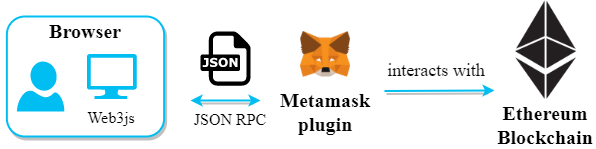
\includegraphics[height=!,width=1\linewidth,keepaspectratio=true]{figures/architecture_of_dapp.png}
    \caption{{\footnotesize Architecture of DApp}}
    \label{fig:architecture_of_dapp}
\end{figure}

\newpage

\section{OAuth}
- OAuth 2.0 flow and explain

\newpage

\section{Trust Service Provider (TSP)}
- Open Banking flow
- Current TSP in Taiwan
- Three stage table

\newpage

\section{Related works}
In this section, we will provide an overview of related literature about blockchain-based access control, identity management, data sharing, and Open Banking ecosystem.\par
In traditional access control management, the most common solution is PKIs, but it has some concerns about scalability and granularity. Paillisse \emph{et al.}~\cite{paillisse2019distributed} presented a blockchain-based approach to address these problems. They take advantage of blockchain to record and distribute access control policies. Daraghmi \emph{et al.}~\cite{daraghmi2019medchain,daraghmi2019unichain} described a blockchain-based system for electronic medical records and academic records, using blockchain smart contract to manage the data access permission securely and effectively. It also utilizes advanced encryption techniques to protect user's privacy. 
Rouhani \emph{et al.}~\cite{rouhani2020distributed} proposed a distributed Attributed-Base Access Control (ABAC) system that can provide auditing of access attempts. This work has focused on addressing audit and scalability, moreover, they apply the solution to the digital library and improve a lot.
Fu \emph{et al.}~\cite{fu2020soteria} proposed a user rights management system that aims to protect user privacy through enforcing executable sharing agreement. They also adopted multi-layer blockchain architecture to satisfy CAP (consistency, availability, and partition tolerance) theorem.\par

More recent attention has focused on data sharing. The common scenario is Open Banking system since it needs secure identity authentication and the perfect mechanism of user data privacy. With blockchain technology, it can solve the shortcoming of the centralized system and prevent user's data from being breached.
\chapter{System Design}
\label{chapter:design}

\section{Overview}
    \begin{figure}[htb]
        \centering
        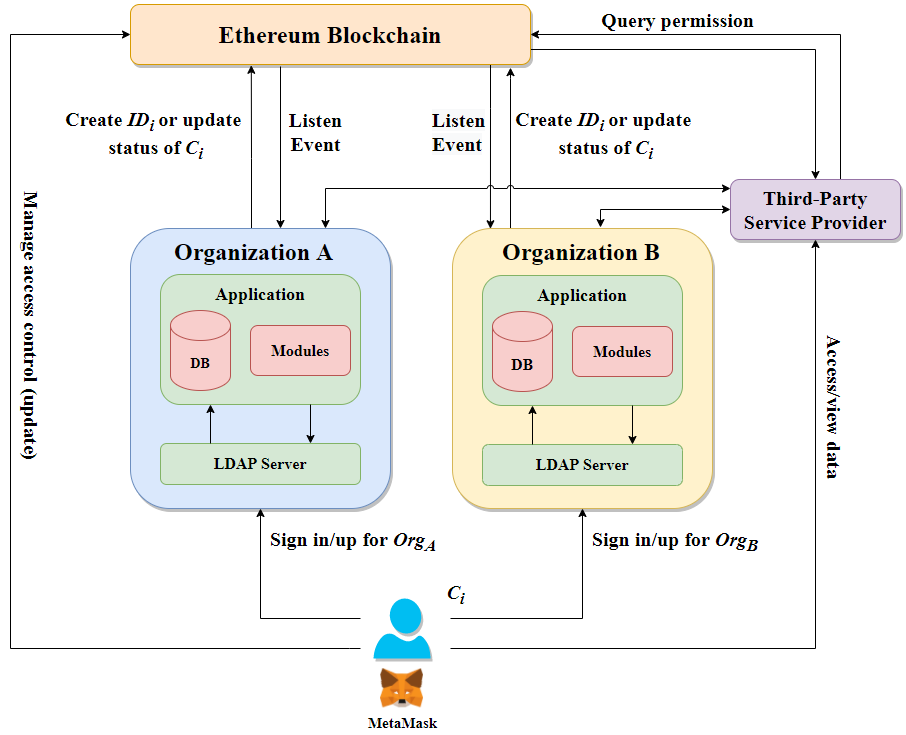
\includegraphics[height=!,width=1\linewidth,keepaspectratio=true]{figures/system_architecture.png}
        \caption{{\footnotesize System Architecture}}
        \label{fig:system_architecture}
    \end{figure}
    The architecture of our system is given in figure~\ref{fig:system_architecture}. Our proposed system solved the account integration and identity verification. And it can apply to various scenarios which need data sharing and distributed access control management such as open banking, medical records, and academic records. At the initial stage, every organization and TSP get an Ethereum account and its corresponding private key to take part in this ecosystem. They must keep their private key safe, or identity theft may occur.  There are several parties in our system: blockchain network, organization, third-party service provider, and user. The interpretation of these parties is stated as following:\par

    \begin{itemize}
        \item \textbf{Blockchain network:} The Ethereum blockchain network is responsible for the user's digital identity and access control management through smart contracts, including identity creation and storage. There have two kinds of contracts to realize that account integration and access manager, detailed in Sect.~\ref{chapter:implementation}.  
        \item \textbf{Organization:} A set of organizations within an ecosystem, identified by the Ethereum account and IP addresses. Each organization represents an independent system, it owns membership software that provides an organization with functionality such as storing and editing member information. The organization not only provides services to customers depend on applications, but also collects user data by using a database. In this paper, organizations provide an interface that users decide to share data.
        \item \textbf{Third-party service provider:} The third-party service provider can be any organization or entity that performs financial services to customer. In this paper, we assume that TSP doesn't manage membership software and they retrieve customer data through blockchain technology.
        \item \textbf{User:} A user owns an organization account and wants to participate in our proposed system. After registering an organization account, the user first needs to pass identity card authentication. Due to the digital identity is unique and important on the smart contract, the organization takes responsibility for ensuring the correct identification card number and the safety of user's personal data. Besides, the user should generate the Ethereum account themself through Metamask.
    \end{itemize}

    \newpage    
\section{Scenario}
    \begin{figure}[htb]
        \centering
        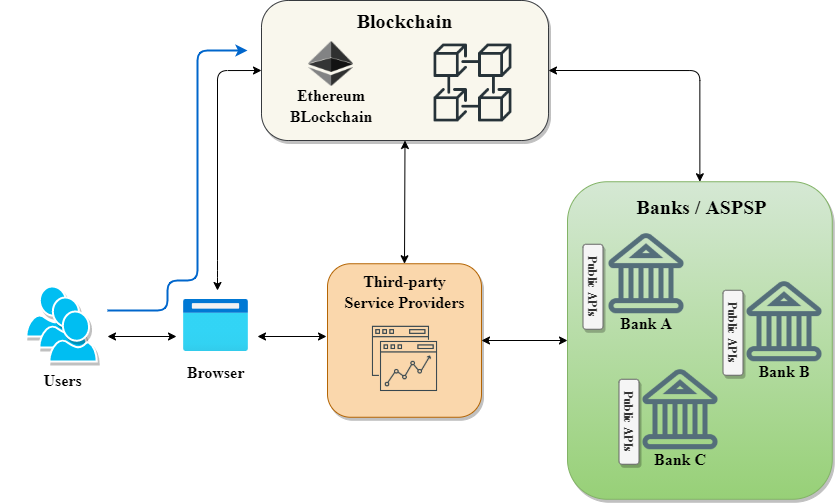
\includegraphics[height=!,width=1\linewidth,keepaspectratio=true]{figures/system architecture-banks.png}
        \caption{{\footnotesize Relation between open banking roles}}
        \label{fig:relation}
    \end{figure}
        From the user perspective, our proposed system provides a single digital identity and access control. The access control for data sharing is constructed using smart contracts. So when banks disclose user's personal data to TSP, banks must have the user's consent through call specific user's smart contract. \par
        In order to apply our proposed system to open banking ecosystem, we have three clearly defined roles: Customer (User), Financial institution, and Third-party services provider. Figure~\ref{fig:relation} gives an overview of our proposed system. It shows the relation between these roles and includes workflows, detailed in Sect.~\ref{ssec:workflow} Each customer interacts with Blockchain by using MetaMask, they not only login with MetaMask but also manage their own access manager contract. That's why customers can allow the specific party to access their data.
    
\section{Workflow} \label{ssec:workflow}
    \subsection{Identity verification}
    \subsection{Account binding}
    \subsection{Third-party login with Ethereum account}
    \subsection{Data sharing}
\chapter{Implementation} 
\label{chapter:implementation}
This chapter describes the design of smart contracts and provides the detailed implementation of each function that is adopted in this paper. The smart contract diagram as shown in Figure~\ref{fig:smart_contract_diagram},  all of the organizations have common \(OMgr\) for managing users' information and storing users' status. The ecosystem initiator enables blockchain-based functionality by deploying a \(OMgr\). It offers application binary interface (ABI) files for all participants to easily call smart contract functions.

\begin{figure}[hb]
    \centering
    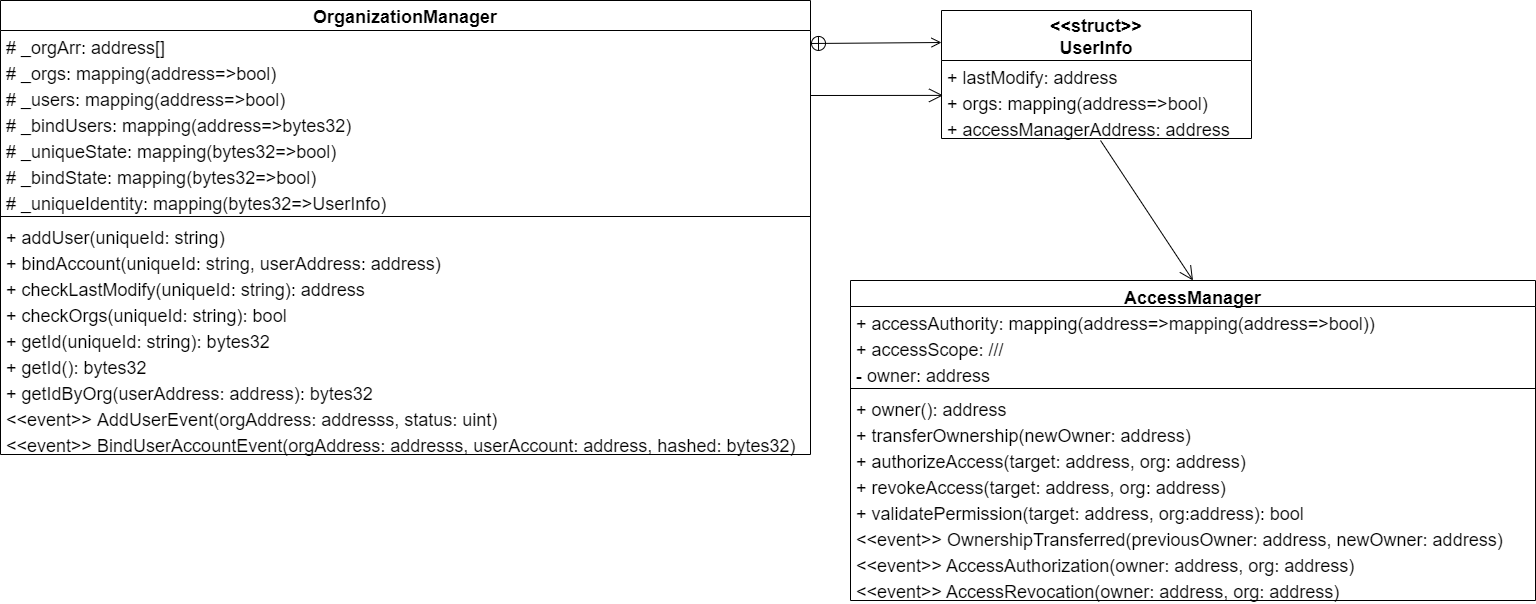
\includegraphics[height=!,width=1\linewidth,keepaspectratio=true]{figures/smart_contract_diagram.png}
    \caption{{\footnotesize Smart Contract Diagram}}
    \label{fig:smart_contract_diagram}
\end{figure}
\section{Smart contract design}
\subsection*{Organization Manager}
The \(OMgr\) is used to manage information that is related to users and organizations, i.e., it records data attributes, users' identity hash value. In Table~\ref{table:userinfo}, the \textit{UserInfo} structure represents an independent \(DI\). After the identity verification process is done as shown in Figure~\ref{fig:identityVerification}, the \(DI\) will be created for users automatically.

\begin{table}[h]
     \centering
     % [] 顯示在 list of tables 的文字
     % {} 顯示在表格上方的文字
     \caption[Table of UserInfo structure]{Table of \textit{UserInfo} structure}
     \label{table:userinfo}
     \begin{tabular}{lll}
     \toprule[1.1pt]
                   Variable & Type & Description\\
     \midrule[1.1pt]
     \textit{lastModify}     & address   & \begin{tabular}[c]{@{}l@{}} Address of last organization that\\ verifies the user\end{tabular}\\                                
     \midrule
     \multirow{1}{*}{\textit{orgs}} & mapping(address==>bool) & Organization's mapping\\
     \midrule
     \multirow{1}{*}{\textit{userAddress}} & address & Corresponding Ethereum address\\
     \midrule
     \multirow{1}{*}{\textit{accessManagerAddress}} & address & Address of $ACMgr_i$ contract\\          
     \bottomrule[1.1pt]
     \end{tabular}
     \end{table}

This smart contract provides several functions to create user identity, bind account with Ethereum address, and create exclusive \(ACMgr\) for the user. And it also defines events in order that the smart contract can emit events to record logs on the block. That enables traceability of identity creation processes. The most important functions we used in \(OMgr\) are \textit{addUser}, \textit{bindAccount} and only the legitimate organizations are able to trigger these functions.\par 
The function \textit{addUser} is invoked after finishing identity verification, the \(OMgr\) check whether the \(ID\) exist on the blockchain. Then if the \(ID\) is new one, the \(OMgr\) will create \textit{UserInfo} for users. Otherwise, the \(OMgr\) will append the address of \(Org\) who triggers this function to the variable \textit{orgs} in \textit{UserInfo}.

\begin{figure}[hb]
    \centering
    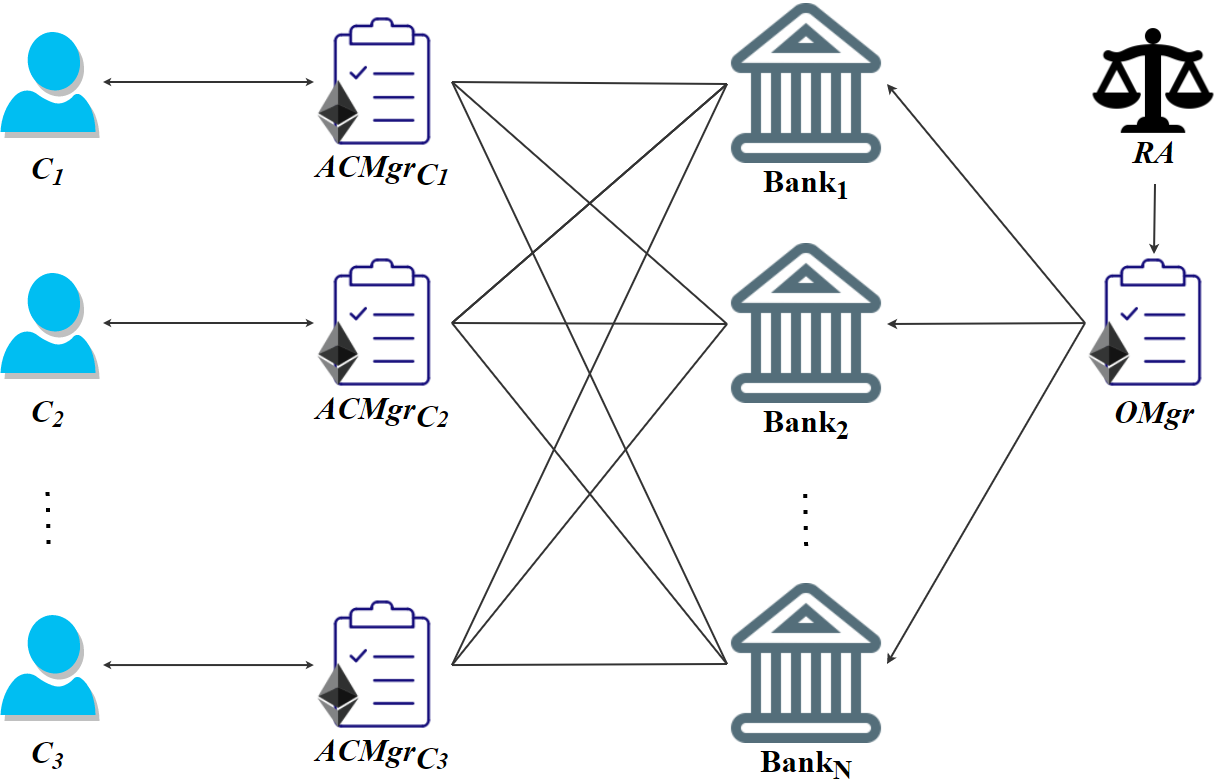
\includegraphics[height=!,width=0.8\linewidth,keepaspectratio=true]{figures/smart_contract_deployment.png}
    \caption{{\footnotesize The relation between smart contracts}}
    \label{fig:smart_contract_deployment}
\end{figure}

\subsection*{Access Manager}
Each user manages access control list of data.
// data structure

\section{Third Party Login}
\section{Integration Account}
\section{Data Sharing}
\section{Token design}
// jwt format(including iss, sub, hashed)
\section{Data privacy protection}
// which data will be save in BC and in DB.
\chapter{Experimental Case Study} 
\label{chapter:related_work}

Here are the experimental case study
\chapter{DApp design and implementation} 
\label{chapter:introduction}

\section{User Registration \& Sign in}
\begin{figure}[htb]
    \centering
    \frame{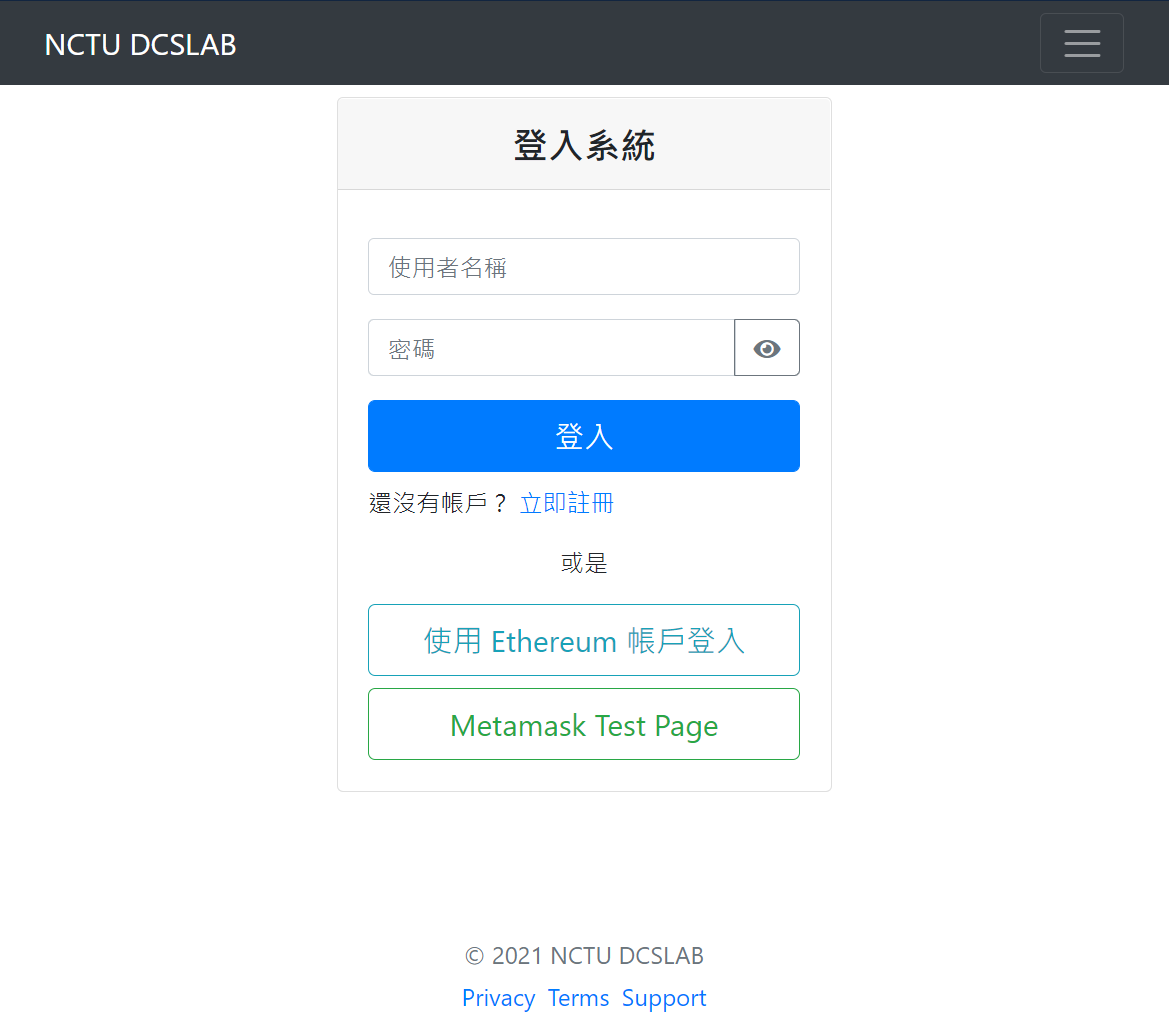
\includegraphics[height=!,width=0.8\linewidth,keepaspectratio=true]{figures/screenshot_signin.png}}
    \caption{{\footnotesize Screenshot of sign in page}}
    \label{fig:signin}
\end{figure}

A user in our proposed system must register as a member of any \(Orgs\) and provider his identification number as indicated in the Figure~\ref{fig:signup}. Afterwards, if the user wants to activate the third-party login, he submits a binding request after the login. As shown in the Figure~\ref{fig:signinblockchain} below, the user clicks on the "Login with Ethereum account" button and the MetaMask signature request will appear to ask the user for confirmation. The purpose of this step is to ensure that the user has ownership of the Ethereum account.
\begin{figure}[h]
    \centering
    \frame{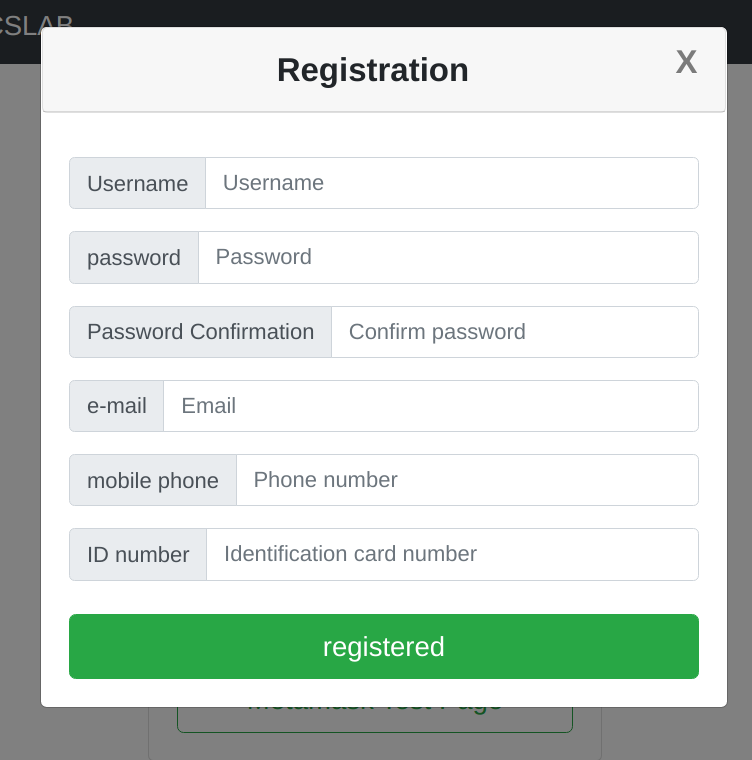
\includegraphics[height=!,width=0.75\linewidth,keepaspectratio=true]{figures/screenshot_signup.png}}
    \caption{{\footnotesize Screenshot of sign up window}}
    \label{fig:signup}
\end{figure}

\begin{figure}[h]
    \centering
    \frame{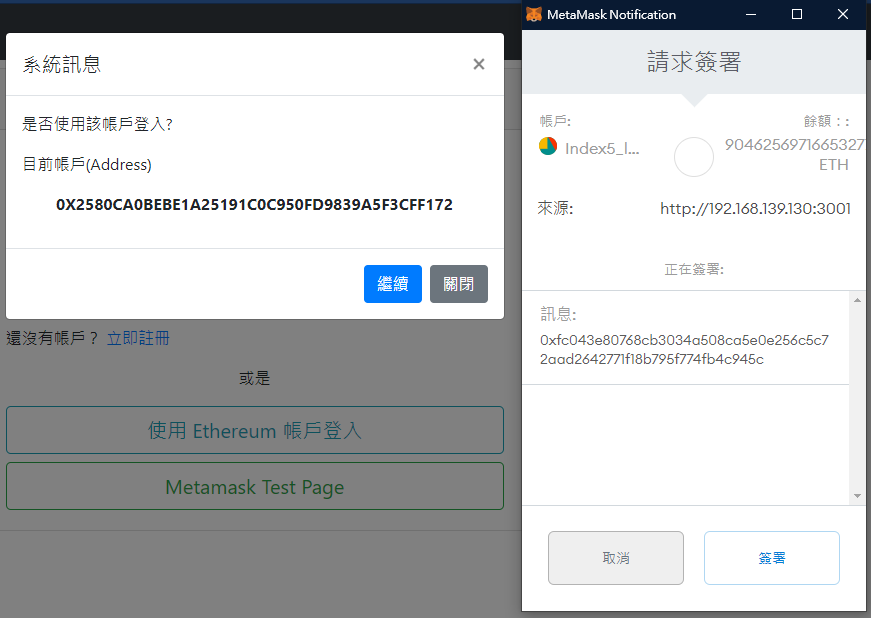
\includegraphics[height=!,width=0.75\linewidth,keepaspectratio=true]{figures/screenshot_thirdpartysignin.png}}
    \caption{{\footnotesize Screenshot of sign in with blockchain}}
    \label{fig:signinblockchain}
\end{figure}
\clearpage
\newpage

\section{User's Profile}

\begin{figure}[htb]
    \centering
    \frame{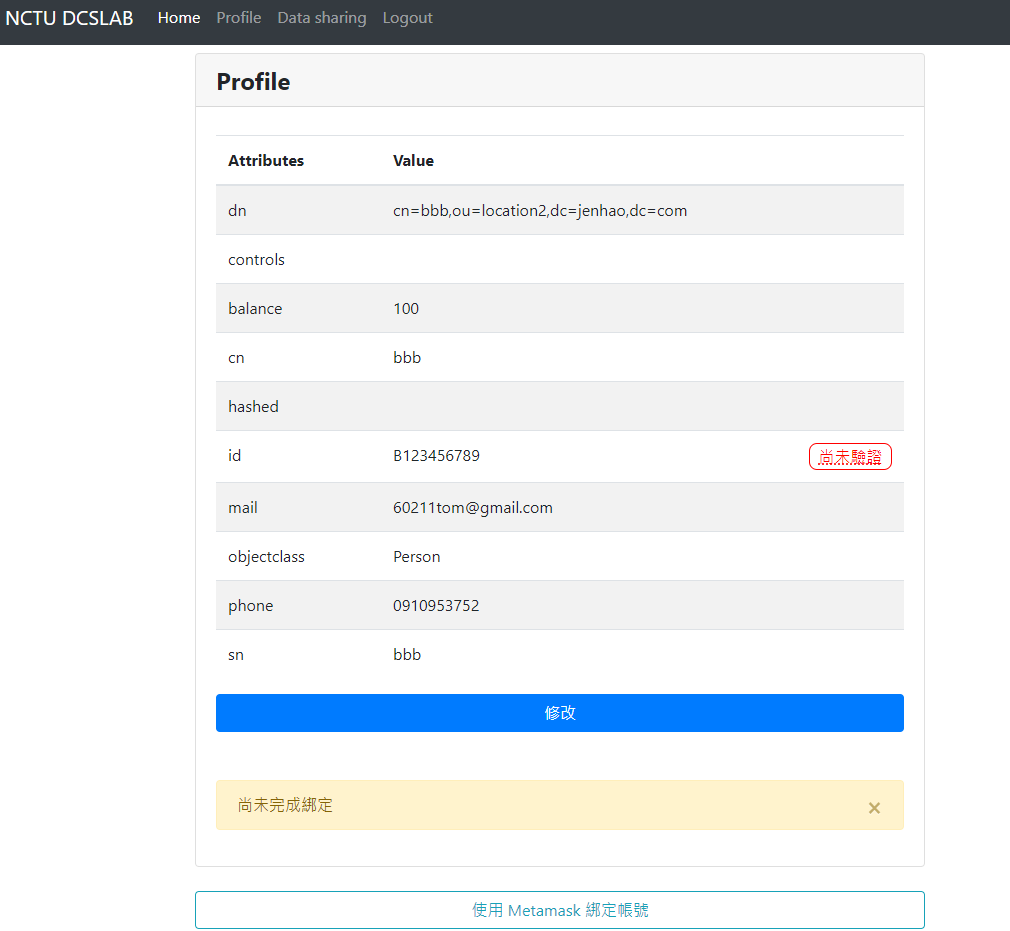
\includegraphics[height=!,width=0.9\linewidth,keepaspectratio=true]{figures/screenshot_profile.png}}
    \caption{{\footnotesize Screenshot of user's profile}}
    \label{fig:profile}
\end{figure}
After the user log in to the Org's service, the user can view their own full profile. Since our implementation adopted the Lightweight Directory Access Protocol (LDAP) to authenticate users, it has stored and retrieved user information from a hierarchical directory structure. As shown in Figure~\ref{fig:profile}, these attributes are parts of the X.500 directory specification, which defines nodes in an LDAP directory. E.g., \textit{dn} (distinguished name), \textit{cn} (common name). In this paper, we also define custom attributes such as \textit{balance}, \textit{hashed}.
\newpage

\begin{figure}[htb]
    \centering
    \frame{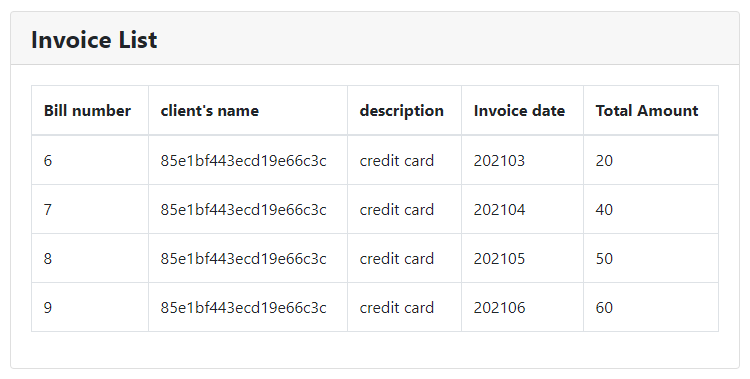
\includegraphics[height=!,width=0.8\linewidth,keepaspectratio=true]{figures/screenshot_invoicelist.png}}
    \caption{{\footnotesize Screenshot of user's invoice list}}
    \label{fig:invoicelist}
\end{figure}

\begin{figure}[htb]
    \centering
    \frame{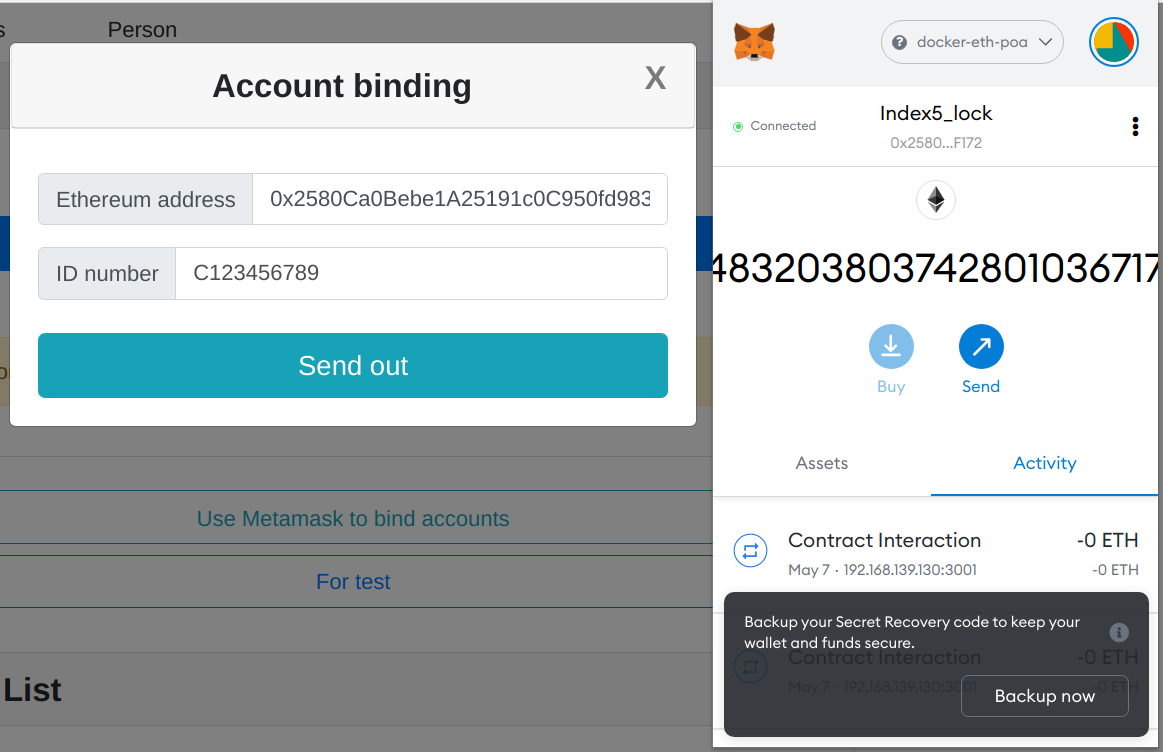
\includegraphics[height=!,width=0.8\linewidth,keepaspectratio=true]{figures/screenshot_bindconfirm.png}}
    \caption{{\footnotesize Screenshot of binding process}}
    \label{fig:bind}
\end{figure}
Besides, we define the user's bill information, the primary key of this information is his name, each user can view their own bill information as shown in Figure~\ref{fig:invoicelist}. So far, we have known two kinds of user information (balance, bill). Even if the user is not involved in a blockchain ecosystem, the user can still see their information.

\clearpage
\newpage

\section{Data sharing}

\begin{figure}[htb]
    \centering
    \frame{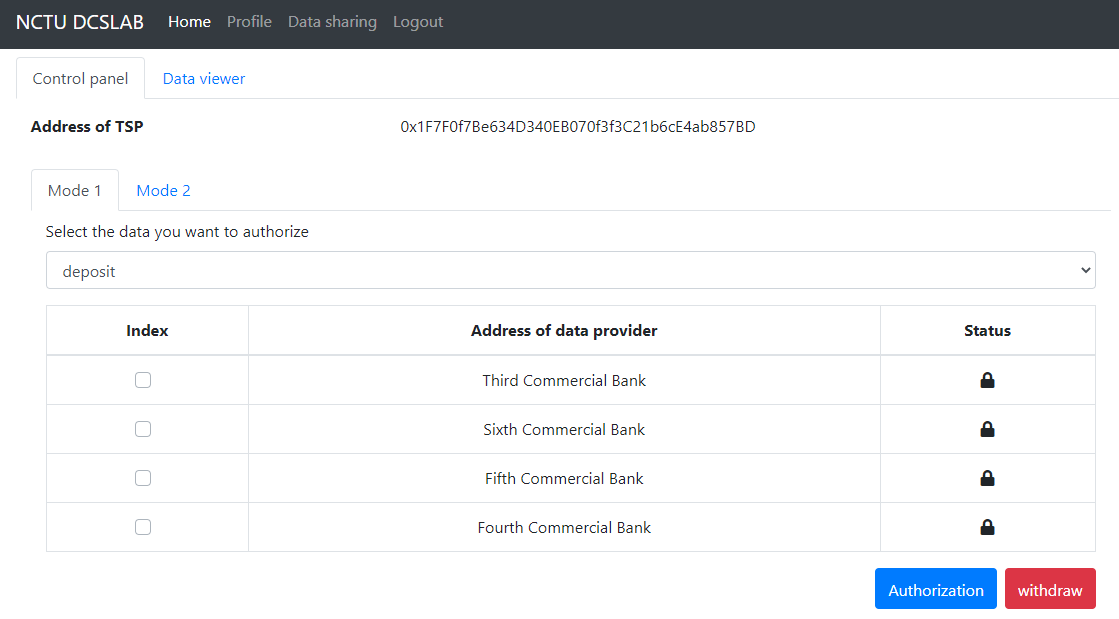
\includegraphics[height=!,width=0.8\linewidth,keepaspectratio=true]{figures/screenshot_controlpanelmode1.png}}
    \caption{{\footnotesize Screenshot of user's control panel with mode 1}}
    \label{fig:mode1}
\end{figure}

\begin{figure}[htb]
    \centering
    \frame{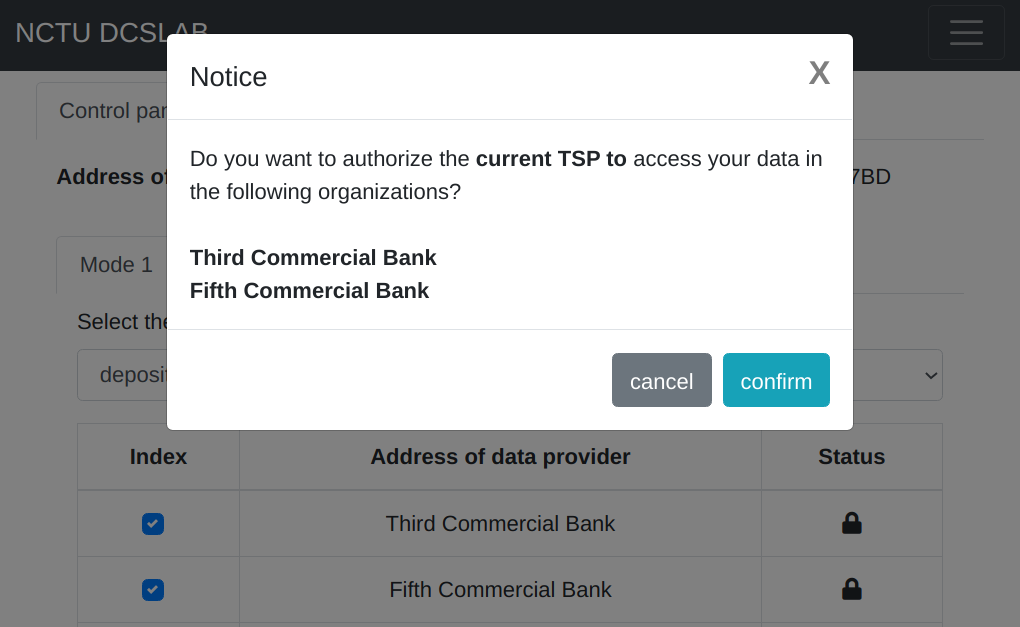
\includegraphics[height=!,width=0.8\linewidth,keepaspectratio=true]{figures/screenshot_authconfirm1.png}}
    \caption{{\footnotesize Screenshot of user's confirmation with mode 1}}
    \label{fig:mode1confirm}
\end{figure}

We provide a web-based user interface (see Figure~\ref{fig:mode1},~\ref{fig:mode2}) for users to control their data access. A user can authorize or revoke access permission at any time through the control panel of this website (see Figure~\ref{fig:mode1confirm}). Although this control panel is provided by the TSP, the TSP will not make access decisions on behalf of the user and the user can interact with web3 on the front-end side via MetaMask to connect to the specific Ethereum node.

\begin{figure}[htb]
    \centering
    \frame{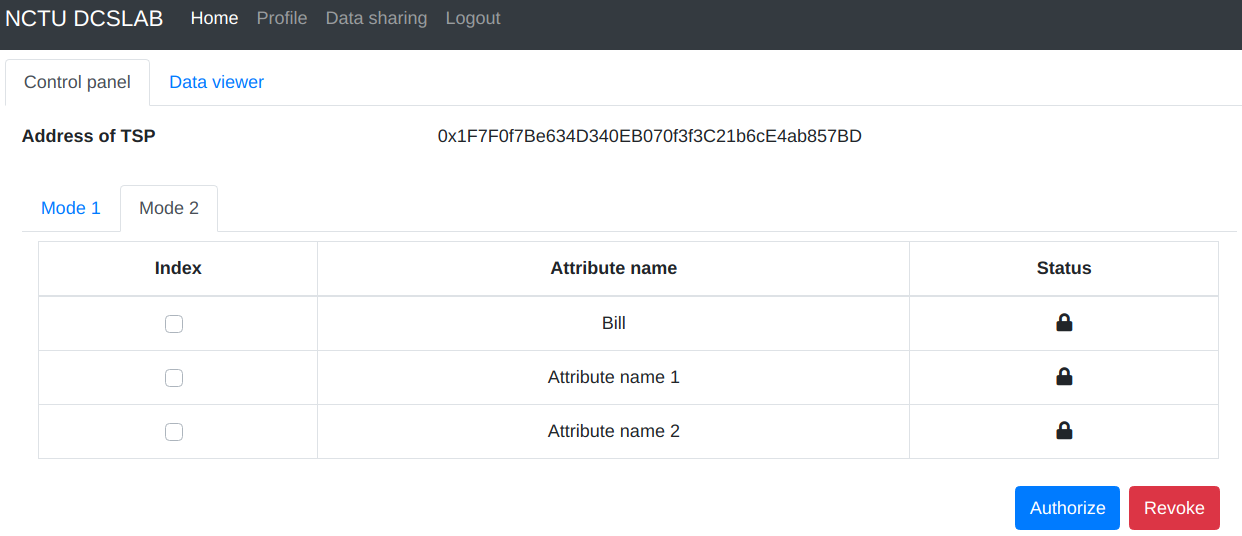
\includegraphics[height=!,width=0.9\linewidth,keepaspectratio=true]{figures/screenshot_controlpanelmode2.png}}
    \caption{{\footnotesize Screenshot of user's control panel with mode 2}}
    \label{fig:mode2}
\end{figure}

\begin{figure}[htb]
    \centering
    \frame{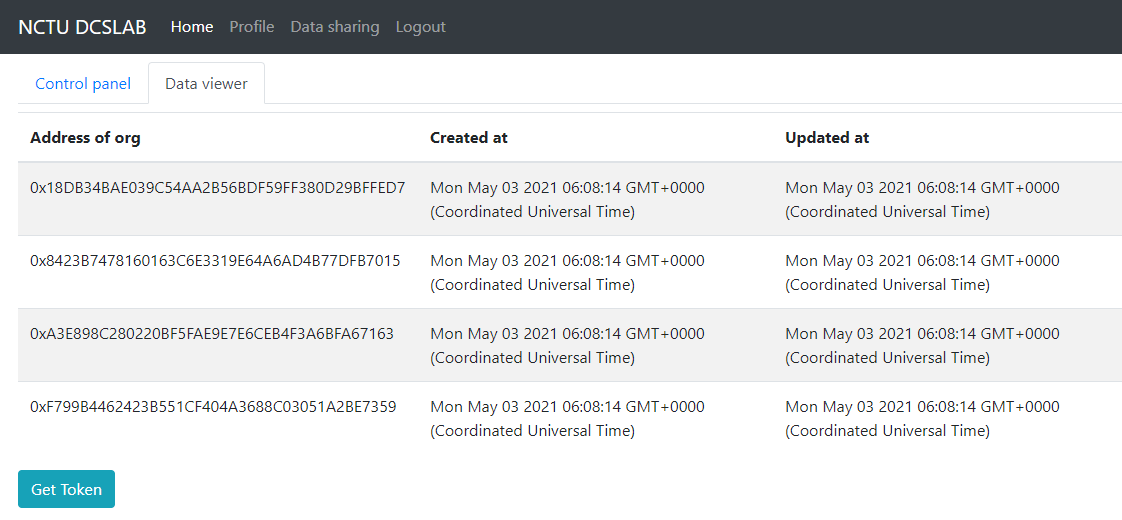
\includegraphics[height=!,width=0.9\linewidth,keepaspectratio=true]{figures/screenshot_requestJWT.png}}
    \caption{{\footnotesize Screenshot of JWTs that already stored in TSP}}
    \label{fig:sreenshotJWT}
\end{figure}
Once the access decision had been made, the user clicks on the "Get token" button to inform the TSP to request for JWTs, and then the user can view the number of JWTs that the TSP got. So that the user can trace how many JWTs are issued by banks.

\section{\textit{Org} \& \textit{TSP}}
In our implementation, an employee of the TSP and Org have to verify users' identity, so they need a web-based user interface to interact with web3 as well. The main difference lies in the architecture. As shown in the Figure~\ref{fig:verifyID}, the control panel only for employees of \(TSP\) or \(Org\).

\begin{figure}[htb]
    \centering
    \frame{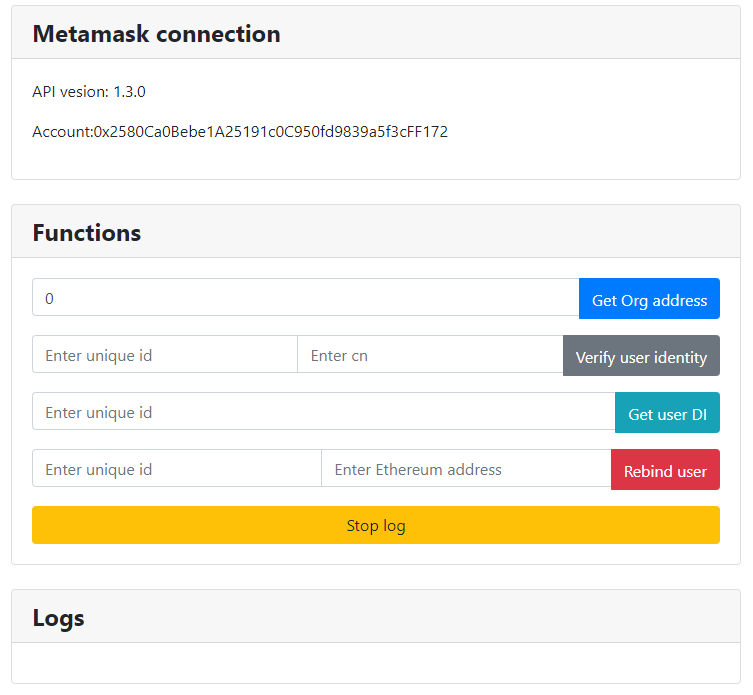
\includegraphics[height=!,width=0.75\linewidth,keepaspectratio=true]{figures/screenshot_verifyID.png}}
    \caption{{\footnotesize Screenshot of organization's administrator}}
    \label{fig:verifyID}
\end{figure}

\begin{figure}[htb]
    \centering
    \frame{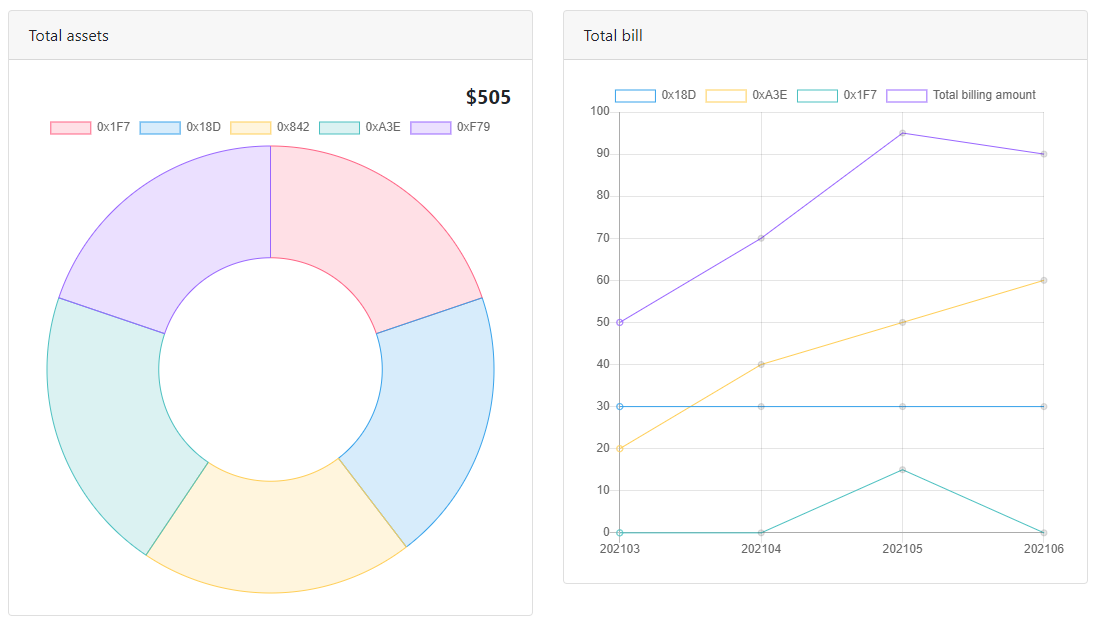
\includegraphics[height=!,width=1\linewidth,keepaspectratio=true]{figures/screenshot_tspresult.png}}
    \caption{{\footnotesize Screenshot of result that TSP generated}}
    \label{fig:result}
\end{figure}
\chapter{Experimental Evaluation}
\label{chapter:evaluation}

Here is the evaluation.
��\begin{table}[h]

    \centering

    % [] o�:y?���� list of tables ??????��?

    % {} o�:y?����h�<h
N�e??????��?

    \caption[Experimental setup]{Experimental setup}

    \label{table:setup}

    \begin{tabular}{p{45mm}p{50mm}}

    \toprule[1.1pt]

    \multirow{1}{*}{Number of organizations} & 5\\

    \midrule

    \multirow{1}{*}{Number of nodes} & 2\\

    \midrule

    \multirow{1}{*}{Number of sealers} & 1\\    

    \midrule    

    \multirow{1}{*}{State database} & LevelDB, key-value storage\\

    \midrule

    \multirow{1}{*}{Consensus mechanism} & Proof of authority (PoA)\\

    \midrule

    \multirow{1}{*}{Block time} & 1s\\

    \midrule

    \multirow{1}{*}{Difficulty} & 0x1\\

    \bottomrule[1.1pt]

    \end{tabular}

    \end{table}
\section{Gas consumption}
\begin{table}[h]
    \centering
    % [] 顯示在 list of tables 的文字
    % {} 顯示在表格上方的文字
    \caption[Gas consumption]{Gas consumption}
    \label{table:gasUsed}
    \begin{tabular}{p{45mm}p{30mm}}
    \toprule[1.1pt]
    Function/Contract   & Gas used\\
    \midrule[1.1pt]
    \multirow{1}{*}{AddUser-create} & 97574\\
    \midrule
    \multirow{1}{*}{AddUser-append} & 36435\\
    \midrule
    \multirow{1}{*}{Bind} & 1390534\\
    \midrule
    \multirow{1}{*}{Authorize} & 49263\\
    \midrule
    \multirow{1}{*}{Revoke} & 19284\\
    \midrule
    \multirow{1}{*}{Authorize-all} & 46580\\    
    \midrule
    \multirow{1}{*}{Revoke-all} & 16625\\
    \midrule
    \multirow{1}{*}{New $Omgr$} & 4494629\\
    \midrule
    \multirow{1}{*}{New $ACMgr$} & 1660077\\    
    \bottomrule[1.1pt]
    \end{tabular}
    \end{table}

\section{Throughput}
\begin{figure}[htb]
    \centering
    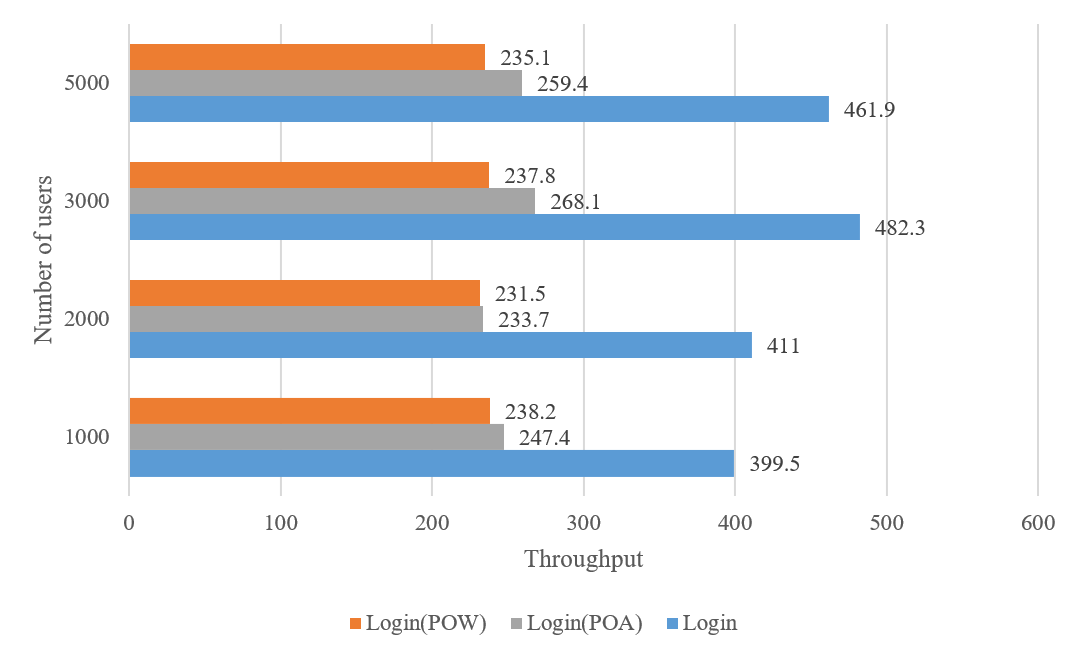
\includegraphics[height=!,width=0.9\linewidth,keepaspectratio=true]{figures/login-throughput.png}
    \caption{{\footnotesize Number of users vs throughput}}
    \label{fig:loginThroughput}
\end{figure}

\begin{figure}[htb]
    \centering
    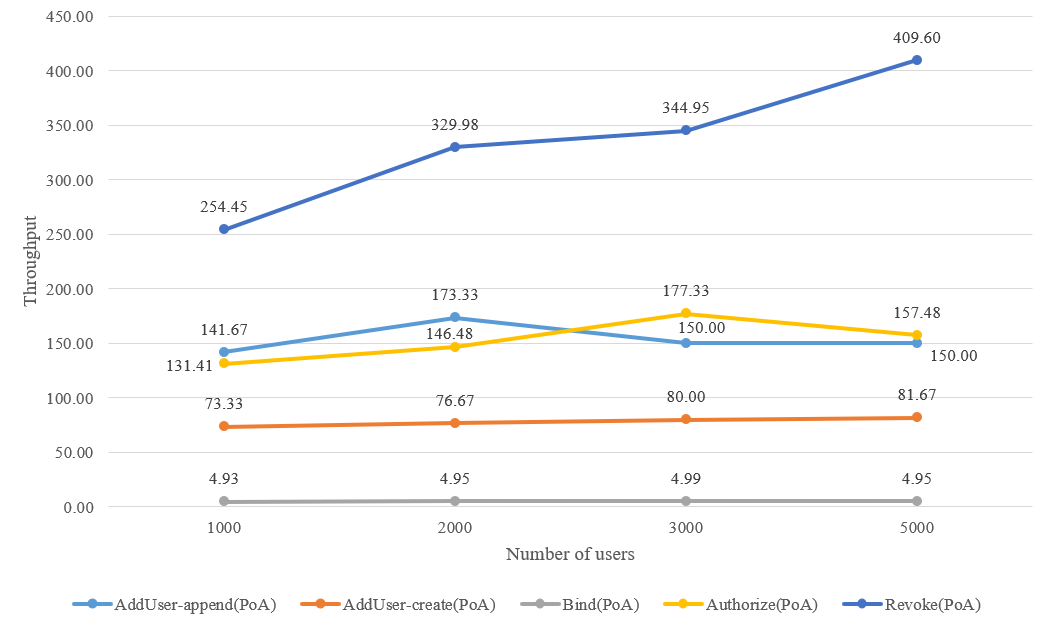
\includegraphics[height=!,width=1\linewidth,keepaspectratio=true]{figures/smart_contract_tps.png}
    \caption{{\footnotesize Each function of smart contract}}
    \label{fig:contract_tps}
\end{figure}

\begin{figure}[htb]
    \centering
    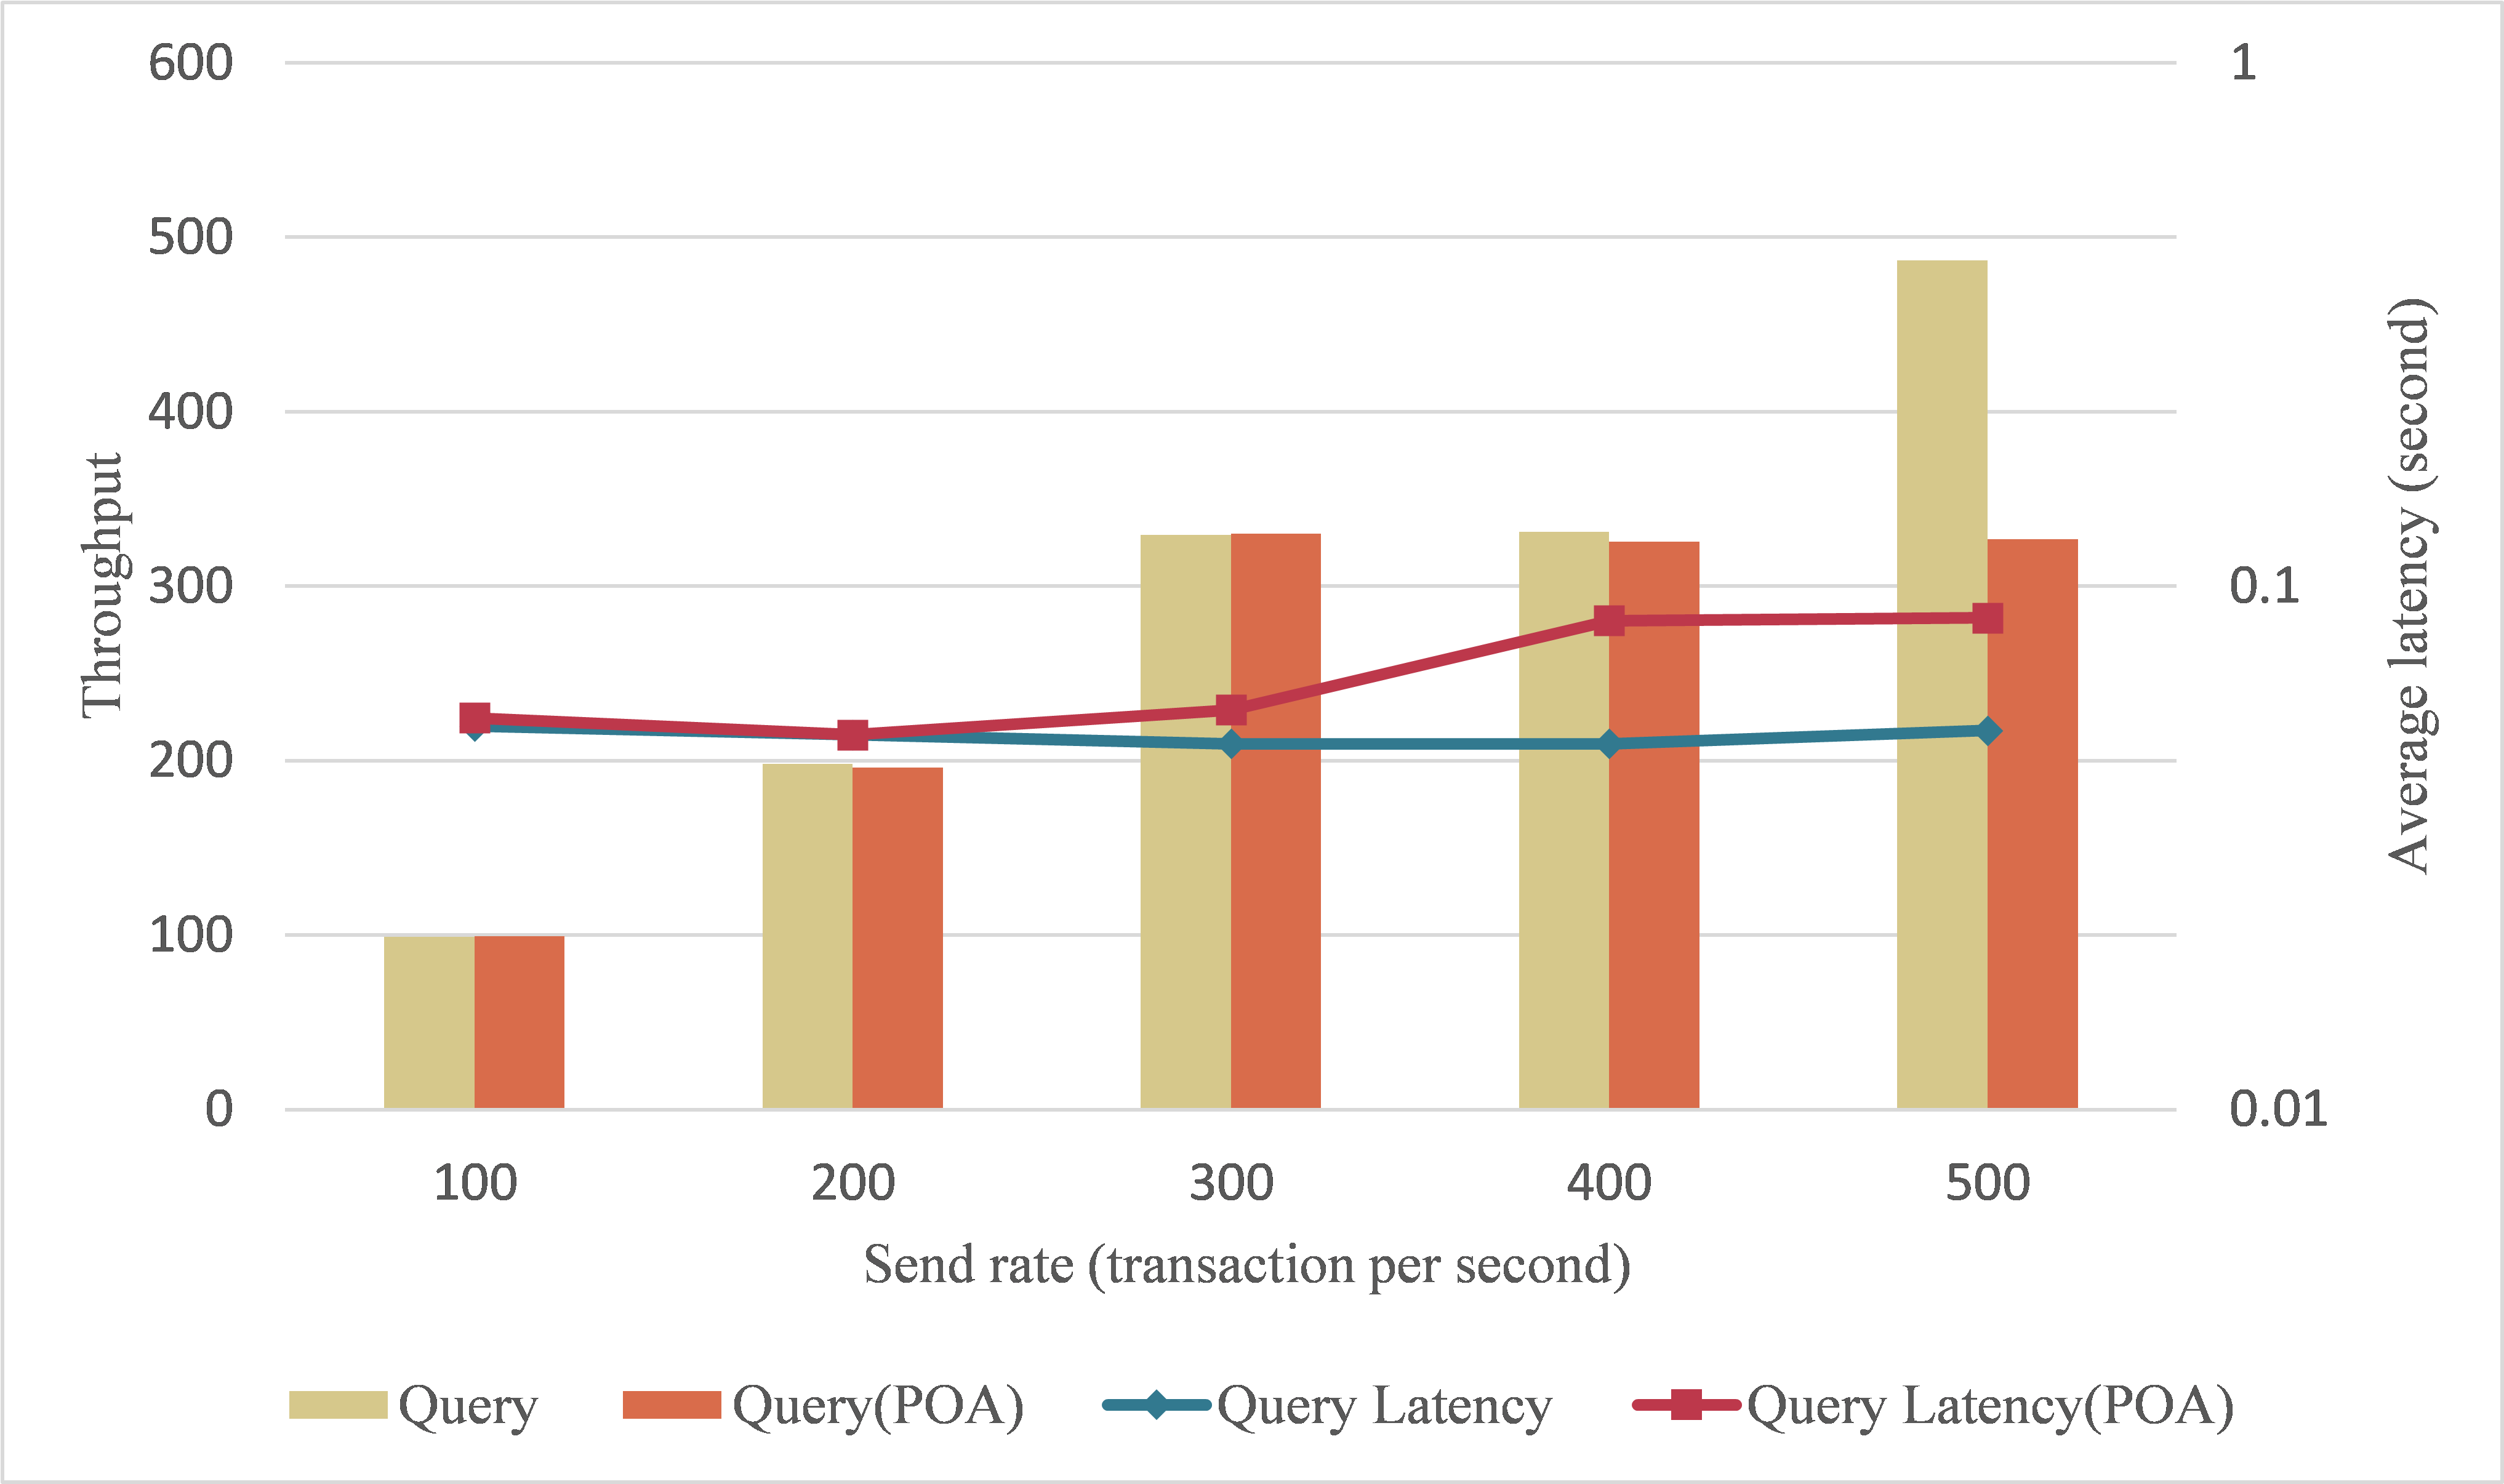
\includegraphics[height=!,width=1\linewidth,keepaspectratio=true]{figures/query.png}
    \caption{{\footnotesize Query with JWT and blockchain}}
    \label{fig:query}
\end{figure}
\chapter{Discussion}
\label{chapter:discussion}

In this chapter, we will first discuss the characteristics of our proposed framework and the related issue of the centralized system. Then we will describe how applications provided by different industries apply this framework.
\par
Firstly, the users and organization administrators can create Ethereum accounts as digital identities by using crypto wallets or tools. The private key of this account can be used in any blockchain network to initiate transactions or triggered contracts, but balances and smart contracts are independent in different chains.   Secondly, the users have a better experience when using DApp because of account integration. For example, users can access their financial data from different banks through blockchain-based login without remembering bank account and password.


\chapter{Conclusion}
\label{chapter:conclusion}

Here is the conclusion.
% \chapter{Introduction}
\label{chapter:intro}

本 template 參考國立交通大學註冊組所提供的 ``學位論文格式" (http://aadm.nctu.edu.tw/registra/form.aspx) 寫成.
因為本 template 使用 XeCJK 來提供中文的論文寫作環境, 所以必須使用 XeLaTeX 編譯.

\section{環境設定}

推薦使用的編譯環境 (LaTeX core + LaTeX editor + Bibliography editor)

\begin{itemize}
\item \textbf{Windows \& Linux}: TeX Live + TeXmaker + JabRef
\item \textbf{Mac OS X}: MacTeX + TeXShop + JabRef
\end{itemize}

\section{開使寫作}

請用你的 LaTeX editor 打開 ``\textbf{main.tex}".
\textbf{main.tex} 是本 template 的主文件 (本文件亦是由編譯 main.tex 產生).
請在 \textbf{main.tex} 加入新的 chapter, 或是由此開啟其他的 chapter files or configuration files (如果你使用的 editor 支援的話), etc.

\section{編譯}

\subsection{編譯指令}

編譯此 template 需要使用 \textbf{XeLaTeX} 和 \textbf{BibTeX} 兩個指令.

\begin{itemize}
\item XeLaTeX (負責編譯 .tex 檔)\\
xelatex -synctex=1 \textbf{-shell-escape} -interaction=nonstopmode \%.tex
\item BibTeX (負責編譯 Bibliography .bib 檔)\\
bibtex \%.aux
\end{itemize}

因大部分的 LaTeX editor 預設的編譯快速鍵是執行 latex, 所以我們需要修改預設的編譯指令.
以下以\textbf{Texmaker}為例, 介紹如何修改:
\begin{enumerate}
\item ``Options" $\rightarrow$ ``Configure Texmaker" $\rightarrow$ ``Commands\\
修改 XeLaTeX 欄位, 加入 ``\textbf{-shell-escape}", 其結果如上所示.
\item ``Options" $\rightarrow$ ``Configure Texmaker" $\rightarrow$ ``Quick Build"\\
勾選 ``XeLaTeX + View PDF"

\end{enumerate}

加入 ``\textbf{-shell-escape}" 是為了讓 XeLaTeX 在編譯時能根據目前執行平台的作業系統 (Windows/Linux/Mac OS X)自動選擇字型.
(各平台預設使用的字型請參考 Section~\ref{sec:fonts})
當你和你的指導教授使用不同的作業系統編寫 LaTeX 時 (尤其當你們還使用 git 之類的版本管理工具來管理論文時), 相信這個小功能可以減少不少修改字型設定的困擾.

\subsection{編譯 main.tex}

\paragraph{編譯順序:} (\textbf{注意}: BibTeX 執行完後, 要執行 XeLaTeX 兩次)

\hspace{2em} \textbf{XeLaTeX} $\rightarrow$ \textbf{BibTeX} $\rightarrow$ \textbf{XeLaTeX} $\rightarrow$ \textbf{XeLaTeX}

\paragraph{使用 Command line:} 我提供了一個簡單的 Makefile, 請執行

\hspace{2em} \textbf{\$ make}

\paragraph{使用 LaTeX Editor:}
Texmaker 提供了兩個編譯快速鍵: XeLaTeX (\textbf{F1}) 和 BibTeX (\textbf{F11}).
在 Texmaker 中編譯請執行:

\hspace{2em} \textbf{F1 $\rightarrow$ F11 $\rightarrow$ F1 $\rightarrow$ F1}

\paragraph{小技巧:} 每次用 \textbf{Texmaker} 開啟 \textbf{main.tex} 後, 請執行 ``Options" $\rightarrow$ ``Define Current Document as `Master Document' ", 將\textbf{main.tex} 設成 XeLaTeX 編譯的主文件, 避免每次編譯時都要切換回 main.tex 才能編譯.

\section{Synopsis}

Chapter~\ref{chapter:doccls} introduces thesis.cls document class.
Chapter~\ref{chapter:secorder} introduces section ordering.
Chapter~\ref{chapter:ref} and~\ref{chapter:fig} explain how to load citation, figures and tables (not completed).
% \chapter{thesis.cls 簡介}
\label{chapter:doccls}

\textbf{thesis.cls} 是本 template 的核心, 其主要功能是產生論文的封面, 設定版面與章節樣式, 並提供自動選擇字型的功能.
因大部分需要使用者輸入的資訊(e.g. author name)都有拉出對應的變數讓使用者設定, 因此
絕大部分的情況下, 你是不需要動到 thesis.cls 的.
當然, 如果你有發現 bug 或是覺得哪些地方有更好的寫法, 也請麻煩在 github 上發個 issue 告訴我吧, 謝謝!

以下介紹如何設定封面資訊與字型, thesis.cls 提供的 options, 以及摘要等檔案放置的位置.

\section{封面資訊}

封面資訊的設定指令全部都放在 \textit{config/frontmatters.tex} 中, 請在此設定你論文的 title, author name, (co-)advisor name, college name (院), institute name (所), field (領域), 日期等資訊.

\textbf{注意:} 如果沒有共同指導教授, \textbackslash coadvisorA, \textbackslash coadvisorAzh, \textbackslash coadvisorB \textbackslash coadvisorBzh 的\{ \}請留白.

\section{字型設定}
\label{sec:fonts}

為了避免在不同作業系統上編譯文件時要重新設定中文字型, thesis.cls 提供了自動選擇字型的功能.
(請在 xelatex 加入 \textbf{-shell-escape} 才能開啟此功能)

\subsection{預設英文字型}

thesis.cls 預設的英文字型在全部作業系統上皆為
\begin{itemize}
\item 本文字型(main font): \textbf{Times New Roman}
\item 無襯線字型(sans-serif font): \textbf{Arial}
\end{itemize}

\subsection{預設中文字型}

thesis.cls 預設的中文字型則詳列於 Table~\ref{table:zhfonts}.
簡單來說, 本文使用``標楷體", 封面字型則使用``明體".

% table 
\begin{table}[h]
\centering
% [] 顯示在 list of tables 的文字
% {} 顯示在表格上方的文字
\caption[Default Chinese font settings]{預設的中文字型}
\label{table:zhfonts}
\begin{tabular}{@{}lll@{}}
\toprule
作業系統     & 本文字型     & 明體字 (用於封面) \\ \midrule
Windows  & 標楷體      & 新細明體       \\
Linux    & AR PL 中楷 & AR PL 明體   \\
Mac OS X & 楷體-繁     & 儷宋 Pro     \\ \bottomrule
\end{tabular}
\end{table}

\subsection{修改預設字型}

thesis.cls 提供了以下四個修改預設字型的指令.
\textbf{注意: 如果修改了預設字型, thesis.cls 則不會再根據所處的作業系統自動選擇字型.}
我將此四個指令獨立出來放在 \textit{config/fonts.tex} 裡面.
如果不想修改預設字型, \{ \} 請留白.

\begin{itemize}

\item \textbf{\textbackslash mainfontzh\{\}} 修改預設中文本文字型

\item \textbf{\textbackslash mingfontzh\{\}} 修改預設中文明體字型

\item \textbf{\textbackslash mainfont\{\}} 修改預設英文本文字型

\item \textbf{\textbackslash sansfont\{\}} 修改預設英文無襯線字型

\end{itemize}


\section{Options provided by thesis.cls}

thesis.cls 提供碩士與博士論文模板, 並提供初稿與終稿等選項讓使用者自行印出的版面格式.
thesis.cls 的 options 設定就在 \textbf{main.tex} 的第一行

\textbackslash documentclass[\textbf{<options>}]\{thesis\}

以下介紹 thesis.cls 所提供的 options

\newpage

\subsection{給沒空的人看的無腦版本}

\paragraph{英文碩士論文} 請設定

\begin{itemize}
\item 初稿\\
\textbackslash documentclass[]\{thesis\}
\item 終稿\\
\textbackslash documentclass[watermark,final]\{thesis\}
\item 只顯示論文內文, 附錄, 和 reference\\
\textbackslash documentclass[review]\{thesis\}
\end{itemize}

\paragraph{中文碩士論文} 在 [ ] 中多加一個 `zh' 就會顯示中文的章節編號和標題了, 舉例來說

\begin{itemize}
\item \textbackslash documentclass[zh,watermark,final]\{thesis\}
\end{itemize}


\paragraph{英文博士論文} 請在 [ ] 中多加一個 `phd', 舉例來說

\begin{itemize}
\item \textbackslash documentclass[phd,watermark,final]\{thesis\}
\end{itemize}

\paragraph{中文博士論文} 一樣在 [ ] 中多加一個 `zh' 就可以了, 舉例來說

\begin{itemize}
\item \textbackslash documentclass[phd,zh,watermark,final]\{thesis\}
\end{itemize}

\paragraph{雙面列印} 預設為單面列印, 如果要雙面列印, 請在 [ ] 中加入 'twoside', 比方說

\begin{itemize}
\item \textbackslash documentclass[twoside,phd,watermark,final]\{thesis\}
\end{itemize}

\paragraph{Known Issue!} 在編譯過英文版後, 加入 `zh' 編譯中文版後的\textbf{第一次編譯}時, XeLaTeX 會出錯.
但只要再編譯一次就沒問題了.
也就是說從英文版轉到中文版的編譯步驟變成:

\hspace{2em} \textbf{XeLaTeX} (\textbf{\textit{Failed!}}) $\rightarrow$ \textbf{XeLaTeX} $\rightarrow$ \textbf{BibTeX} $\rightarrow$ \textbf{XeLaTeX} $\rightarrow$ \textbf{XeLaTeX}

\subsection{詳細版的 Class Options}

thesis.cls 提供的 options 詳列於 Table~\ref{table:clsoptions}.
標注 (default) 代表 thesis.cls 的預設值, 不需要寫在 [ ] 內.

% 把 table 的內容放在另一個檔案再 load, 讓 tex 看起來乾淨一點
\begin{table}[h]
\centering
% [] 顯示在 list of tables 的文字
% {} 顯示在表格上方的文字
\caption[Class options provided by thesis.cls]{Class options provided by thesis.cls}
\label{table:clsoptions}
\begin{tabular}{lll}
\toprule[1.1pt]
                      & Options   & Description\\
\midrule[1.1pt]
\multirow{2}{*}{論文類型} & master    & 碩士論文 (default)\\
                      & phd       & 博士論文\\
\midrule
\multirow{3}{*}{論文格式} & draft     & 初稿 (default)\\
                      & final     & 終稿\\
                      & review    & 只顯示內文,參考文獻,與附錄\\
\midrule
\multirow{2}{*}{語言}   & en        & 英文章節編號與標題 (default)\\
                       & zh        & 中文章節編號與標題\\
\midrule
\multirow{2}{*}{列印}   & oneside   & 單面列印 (default)\\

                        & twoside   & 雙面列印\\
\midrule
浮水印                   & watermark & \begin{tabular}[c]{@{}l@{}}review mode 不顯示\\ draft mode 顯示 ``DRAFT" 字樣\\ final mode 顯示指定的浮水印\end{tabular} \\
\midrule
裝訂                    & binding   & \begin{tabular}[c]{@{}l@{}} 在頁面左側預留 1cm 的裝訂空間\\ (enabled by default under final mode)\end{tabular}\\
\bottomrule[1.1pt]
\end{tabular}
\end{table}


\section{論文檔案位置}

Table~\ref{table:pages} 詳列了摘要, 誌謝等頁面的位置.
如果你使用 Texmaker 之類的 editor 的話, 可以從 main.tex 連結到這些檔案.

\textbf{注意:} 題獻頁, 自傳, 著作目錄只有博士論文才需要填寫, 也只有在 \textbackslash documentclass[] 加入 `phd' 選項後才會被編譯.

\begin{table}[h]
\centering
% [] 顯示在 list of tables 的文字
% {} 顯示在表格上方的文字
\caption[檔案位置]{檔案位置}
\label{table:pages}
\begin{tabular}{@{}ll@{}}
\toprule
     & 位置                      \\ \midrule
中文摘要 & abs/abstract\_zh.tex    \\
英文摘要 & abs/abstract\_en.tex    \\
誌謝   & ack/ack.tex             \\
題獻頁  & ack/dedication.tex      \\
自傳   & author/cv.tex           \\
著作目錄 & author/publications.tex \\ \bottomrule
\end{tabular}
\end{table}

至於論文內文的檔案要放哪裡, 則看個人喜好.
我自己的習慣是把論文的每一個 chapter 獨立成一個 .tex 檔, 放在 \textit{chapters/} 下.
而附錄也是寫成獨立的 .tex 檔, 放在另一個資料夾下, 方便管理.
請參考此 template 的 \textit{chapters/} 與 \textit{appx/} 兩個資料夾.

% \chapter{Section Ordering}
\label{chapter:secorder}

Section ordering in \textit{thesis.cls} is:
\begin{itemize}
\item Chapter (shown in \textbf{Table of Contents})
\item Section (shown in \textbf{Table of Contents})
\item Subsection (shown in \textbf{Table of Contents})
\item Paragraph
\item Subparagraph
\end{itemize}
DONOT use \textbackslash subsubsection, it is not supported in \textit{thesis.cls}.
It is replaced by \textbackslash paragraph.

\section{Section}
\label{sec:secorder}
\lipsum[1-2]  % dumy text generator

\subsection{Subsection}
\label{subsec:secorder}
\lipsum[3-4]  % dumy text generator

\paragraph{Paragraph}
\lipsum[5-6]  % dumy text generator

\subparagraph{Subparagraph}
\lipsum[7]  % dumy text generator

\section{Section}
\label{sec:secorder}
\lipsum[8]  % dumy text generator
% \chapter{Reference}
\label{chapter:ref}

Section~\ref{sec:citation} explains how to include citation.
Section~\ref{sec:quote} explains how to use quote.

\section{Citation}
\label{sec:citation}

We use \textbackslash cite\{\} to cite references.
Besides, we need to use $\sim$ to connect \textbackslash cite\{\} and previous text.

For example (請看 .tex 檔),
\begin{itemize}
\item Yang et al.~\cite{Yang_2016} analyzed the strategy and tactics of Reinhard von Lohengramm blablabla.
\item Yang and Fox divides the history of Free Planets into three eras~\cite{Yang_2017}.
\end{itemize}

Note that, when mentioning authors
\begin{itemize}
\item only 1 author: Yang [citation] ...
\item just 2 authors: Yang and Fox [citation] ...
\item more than 2 authors: Yang et al. [citation] ...
\end{itemize}

\section{Quote}
\label{sec:quote}

\textbf{注意:} 在 latex 中使用單/雙引號時要小心, 左邊的引號打法不同 (請看 .tex 檔):
\begin{itemize}
\item `單引號'
\item ``單引號"
\end{itemize}

% \chapter{Figures and Tables}
\label{chapter:fig}

關於怎麼使用圖和表格, 網路上都可以找到許多介紹. Google it.
(其實是我累了, 不想寫了 XD)

\section{Figures}

這裡介紹如何載入一張圖片, 解釋請看 .tex 檔的註解吧!
此外, 我個人習慣是把所有的圖檔都放在一個資料夾下, 像是 \textit{figures/}

\begin{figure}[b]
  \centering
  % 圖片的高度與寬度, height 設為 ! 代表由寬度大小等比例縮放
  \includegraphics[height=!,width=0.4\linewidth,keepaspectratio=true]%
  % 圖片的位置
  {figures/nctu_logo}
  % [] 放的是顯示在 list of figure 的文字
  % {} 放的是顯示在圖下方的文字
  \caption[NCTU logo]{{\footnotesize The history of NCTU days back to 1896 ...}}
  \label{fig:nctu_logo}
\end{figure}

\textbf{注意:} 在呼叫圖的標籤的時候, 請寫 \textbf{Figure$\sim$\textbackslash ref\{label\}}.
(請參考 .tex 檔看我是如何載入 Figure~\ref{fig:nctu_logo} 的吧).

\section{Tables}

我個人的習慣是把表格的內容放到另一個 .tex 內, 再把這些 .tex 檔放到另一個資料夾下 (e.g. \textit{tables/}), 讓本文看起來不會那麼亂.
請參考 Table~\ref{table:clsoptions} 裡面的註解 (檔案位置 \textit{tables/table-classopt.tex}), 看看要怎寫一個簡單的 table 吧.


%-------------------------------------------------------------------------------
% 參考文獻
%-------------------------------------------------------------------------------

% Set bib style
\bibliographystyle{IEEEtran}

% Add Bibliography to "Table of Contents"
\addBibToContents

% Usage:
%   \bibliography{bib/bib1,bib/bib2,...,bib/bibN} % 注意: 不要有空格
%
% For IEEEtran users:
%   DO NOT remove bib/BSTcontrol.bib when using IEEEtran.bst. The reason is that
% when we cite two papers of the same (or similar) authors, IEEEtran.bst would
% replace the author names with "------". To avoid this, we use BSTControl.bib
% to set ctldash_repeated_names to 'no'.
%
% For non IEEEtran users:
%   Please delete bib/ieeeBSTcontrol from \bibliography{}
\bibliography{bib/ieeeBSTcontrol,bib/thesis}

%-------------------------------------------------------------------------------
% 附錄
%-------------------------------------------------------------------------------

% Start appendix
\appendix

% Add appendicies to "Table of Contents"
\addAppxToContents

% 請從此開始依序擺放附錄
\chapter{附錄標題}

\section{Testing}


%-------------------------------------------------------------------------------
% 作者簡歷
%-------------------------------------------------------------------------------

% 簡歷 (Only shown in a PhD dissertation)
\begin{vita}%

{\bf Wen-Li Yang} is a character in Tanaka Yoshiki's science fiction, ``Die Legende der Sternhelden." His research interests include drinking and sleep.

\end{vita}

% 著作列表 (Only shown in a PhD dissertation)
\begin{publications}%

%%%%%%%%%%%%%%%%%%%%%%%%%%%%%%%%%%%%%%%%%%%%%%%%%%%%%%%%%%%%%%%%%%%%%%%%%%%%%%%

\section*{Journal Papers}
\begin{spacing}{1}
\begin{enumerate}

\item {\bf \underline{Wen-Li Yang}}, Bamboo Fox, ``Carry the Free Planets Star Fleet in Three Ways," \textit{Journal of Galaxy}, vol. 9527, no. 1, pp. 22--66, 2016

\end{enumerate}
\end{spacing}

%%%%%%%%%%%%%%%%%%%%%%%%%%%%%%%%%%%%%%%%%%%%%%%%%%%%%%%%%%%%%%%%%%%%%%%%%%%%%%%

\section*{Conference Papers}
\begin{spacing}{1}
\begin{enumerate}

\item {\bf \underline{楊威利}}, 竹狐, ``如何屌打金髮小子," in \textit{International Conference of Military History}, 2016, Iserlohn, Germany

\end{enumerate}
\end{spacing}

%%%%%%%%%%%%%%%%%%%%%%%%%%%%%%%%%%%%%%%%%%%%%%%%%%%%%%%%%%%%%%%%%%%%%%%%%%%%%%%

\end{publications}

\end{document}